\documentclass[10pt]{article}

\usepackage{amsmath}
\usepackage{amsfonts}
\usepackage{amssymb}
\usepackage{gensymb}
\usepackage{fancyhdr}
\usepackage{textpos}
\usepackage{titlesec}
\usepackage[hyphens]{url}
\usepackage[hidelinks]{hyperref}
\usepackage{graphicx}
\graphicspath{ {./images/}}

\newtheorem{theorem}{Theorem}[subsection]
\newtheorem{lemma}[theorem]{Lemma}

\newcommand{\paren}[1]{\left ( #1 \right )}
\newcommand{\set}[1]{\left \{ #1 \right \}}
\newcommand{\floor}[1]{\left \lfloor #1 \right \rfloor}
\newcommand{\ceiling}[1]{\left\lceil #1 \right\rceil}
\newcommand{\cbrt}[1]{\sqrt[3]{#1}}
\newcommand{\dst}{\displaystyle}
\newcommand{\cycsum}{\sum_{\mathrm{cyc}}}
\newcommand{\symsum}{\sum_{\mathrm{sym}}}
\newcommand{\cycprod}{\prod_{\mathrm{cyc}}}
\newcommand{\symprod}{\prod_{\mathrm{sym}}}
\newcommand{\dang}{\measuredangle}
\newcommand{\ray}[1]{\overrightarrow{#1}} 
\newcommand{\seg}[1]{\overline{#1}}
\newcommand{\geoarc}[1]{\wideparen{#1}}
\DeclareMathOperator{\sign}{sgn}
\newcommand{\dg}{^\circ}
\newcommand{\reals}{\mathbb{R}}
\newcommand{\complexes}{\mathbb{C}}
\newcommand{\rationals}{\mathbb{Q}}
\newcommand{\integers}{\mathbb{Z}}
\newcommand{\naturals}{\mathbb{N}}
\newcommand{\field}{\mathbb{F}}

\DeclareMathOperator{\cis}{cis}
\DeclareMathOperator{\lcm}{lcm}

\newcommand{\themonth}{March}
\newcommand{\theyear}{2019}
\newcommand{\theissue}{The Big Document}
\newcommand{\thefirstday}{1}

\newcounter{day}
\setcounter{day}{\thefirstday}
\newcounter{solution}
\setcounter{solution}{1}
\newcounter{datenumber}
\setcounter{datenumber}{26} %starts on the 26th of March

\titleformat{\subsection}[runin]{\normalfont\large\bfseries}{\themonth~\arabic{datenumber}}{1em}{}

\renewcommand{\thesubsubsection}{Solution~\arabic{subsubsection}}

\setcounter{tocdepth}{2}

\pagestyle{fancy}
\fancyhf{}
\fancyhead[L]{\rightmark}
\fancyhead[R]{\theissue}
\cfoot{\thepage}

%Args: Problem # (optional), Source, Category, Statement
\newcommand{\problem}[4][0]{
	\newpage
	\subsection{[#3] \space #2} \hfill 
	{\large\textbf{Day \arabic{day}}} %| \arabic{subsection} \themonth~\theyear
	\begin{flushleft} #4 \end{flushleft}
	\vspace{1em}
	\addtocounter{day}{1}
	\addtocounter{datenumber}{1}
	\setcounter{solution}{1}
}

%Args: Problem # (optional), Sumbitter, UserID, Solution
\newcommand{\solution}[4][0]{
	\paragraph{Solution \arabic{solution}} \hfill submitted by #2 \hfill \texttt{#3}
	\begin{flushleft} #4 \end{flushleft}
	\addtocounter{solution}{1}
	\vspace{1em}
}

%Args: Problem # (optional), Sumbitter, UserID, Solution
\newcommand{\anonsolution}[2][0]{
	\paragraph{Solution \arabic{solution}} 
	\begin{flushleft} #2 \end{flushleft}
	\addtocounter{solution}{1}
	\vspace{1em}
}

\begin{document}
	\begin{titlepage}
		\begin{textblock*}{2cm}(13.75cm,-4cm) \begin{flushright}\theissue \end{flushright} \end{textblock*}
		\vspace*{\stretch{1.0}}
		\begin{center}
			\LARGE\textbf{Mathematical Olympiads\\Discord Server}\\
			\vspace*{\stretch{3.0}}
			\Huge\textbf{POTD Solutions}\\
			\vspace*{\stretch{2.0}}
			\Large\textbf{\theissue}\\
			%\vspace*{\stretch{3.0}}
			%\large\textit{Compiled by server staff}\\
			\vspace*{\stretch{15.0}}
			\Large\textsc{Main Contributors}\\
			\vspace*{\stretch{0.7}}
			\normalsize{brainysmurfs, Daniel, Tony Wang (individual contributors listed next to each problem)}\\
			\vspace*{\stretch{0.7}}
			Discord Server Link: \url{https://discord.gg/m22vNrX}\\
			Problem Spreadsheet: \url{http://bit.ly/potd-history}\\
		\end{center}
		\vspace*{\stretch{2.0}}
	\end{titlepage}
\section{Introduction}

This document is an set of problems and solutions which have been listed in the \texttt{\#problem-of-the-day} channel of the Mathematical Olympiads Discord Server. Problems are selected from past contests and range from very easy to IMO3/6 level and beyond.

Although the document has been compiled by staff, solutions will be typically member-submitted. As these are problems ``of the day'', the set of problems is continually growing and thus solutions are welcome. If you wish to submit a solution, please send a direct message to the bot \texttt{Staff Mail} via the command \texttt{m.submit}. Alternatively, you may submit a pull request on Github. You will be credited if you wish.

The staff team are indebted to \texttt{www.imomath.org} for making available English translations of many national and international Mathematics Olympiads.

\paragraph{Tag system} Each problem is tagged according to its genre and difficulty. Genre is indicated using initials\footnote{\textbf{A}lgebra, \textbf{C}ombinatorics, \textbf{G}eometry, \textbf{N}umber theory and \textbf{C}ombinatorial \textbf{g}eometry.} and difficulty is indicated on a scale with 1 being very easy, 6 being the typical difficulty of an IMO1/4 problem, and 10 being the typical difficulty of an IMO3/6 problem. For example, a problem assigned the [NCg2] tag is an easy problem in number theory involving some combinatorial geometry.\\

Note that this document is a compilation of all the problems ever to be submitted. Monthly releases will also be available. 

\section{Problems}

These begin on the next page.

\problem[1]{2015 Romanian MoM, Q1}{N4}{Does there exist an infinite sequence of positive integers $a_1, a_2, a_3, \dots$ such that $a_m$ and $a_n$ are coprime if and only if $\lvert m - n \rvert = 1$?}

\solution[1]{SharkyKesa}{268970368524484609}{Suppose the primes are $p_1$, $p_2$, $p_3$, ... . Set $$a_1 = p_2 \cdot p_3$$and $$a_n = p_{n+2} \cdot p_{n-1} \cdot p_{n-3} \cdot p_{n-5} \cdots$$ Then it is trivial to show consecutive $a_i$ are co-prime, but the rest are not co-prime.\footnote{It would be great if someone were to provide a solution which explicitly showed how this sequence fulfilled the conditions of the problem.}}

\problem[2]{2018 IMO Shortlist, C1}{C5}{A rectangle $R$ with odd integer side lengths is divided into small rectangles with integer side lengths. Prove that there is at least one among the small rectangles whose distances from the four sides of $R$ are either all odd or all even.}

\solution[2]{SharkyKesa}{268970368524484609}{Colour in chessboard fashion with the corners as black, so the number of blacks is 1 greater than whites. Then there exists an internal rectangle with more blacks than whites, so it must have all corners as blacks, which means it satisfies the property that the distance to the sides is all odd or even.}

\problem[3]{2014 BMO2, Q2}{A4}{Prove that it is impossible to have a cuboid for which the volume, the surface area and the perimeter are numerically equal. (The perimeter of a cuboid is the sum of the lengths of all its twelve edges.)}

\solution[3]{Tony Wang}{541318134699786272}{Let the sides of the cuboid be $a$, $b$ and $c$. Furthermore let $X = abc$, $Y = 2(ab+bc+ca)$, and $Z=4(a+b+c)$. \\
Now suppose that $XZ = Y^2$, from $X=Y=Z$. Then this means that $$
4(a^2bc+b^2ca+c^2ab) = 4(a^2b^2+ab^2c+a^2bc+ab^2c+b^2c^2+abc^2+a^2bc+abc^2+a^2c^2)$$
So $$a^2b^2+ab^2c+b^2c^2+a^2bc+a^2c^2=0$$
Since $a$, $b$, $c > 0$ this is impossible, as required. 
}

\problem[4]{2015 APMO, Q4}{Cg4}{Let $n$ be a positive integer. Consider $2n$ distinct lines on the plane, no two of which are parallel. Of the $2n$ lines, $n$ are colored blue, the other $n$ are colored red. Let $\mathcal{B}$ be the set of all points on the plane that lie on at least one blue line, and $\mathcal{R}$ the set of all points on the plane that lie on at least one red line. Prove that there exists a circle that intersects $\mathcal{B}$ in exactly $2n-1$ points, and also intersects $\mathcal{R}$ in exactly $2n-1$ points.}

\solution[4]{SharkyKesa}{268970368524484609}{Consider the pair of red-blue lines with maximal angle between them, and consider a circle of increasing radius tangent to them through this angle. Trivial angle chasing yields that this circle must eventually intersect every other line (else you get a bigger angle)\footnote{Not rigorous yet. Additions are welcome.}}

\problem[5]{2005 IMO, Q4}{N5}{Determine all positive integers relatively prime to all the terms of the infinite sequence \[a_n=2^n+3^n+6^n -1,\, n\geq 1.\]}

\solution[5]{SharkyKesa}{268970368524484609}{Note that $2 \vert a_1=10$, $3 \vert a_2=48$. Now suppose $p > 3$ and p is prime. Then, 
\begin{equation}
$$\begin{align*}
a_{p-2} &= (3^{p-2} + 1)(2^{p-2} + 1) - 2\\
&= (1/3 + 1)(1/2 + 1) - 2\\
&= 4/3 \times 3/2 - 2 = 2 - 2\\
&= 0 \mod p
\end{align*}$$
\end{equation}
So $p \vert a_{p-2}$. Thus all primes $p$ eventually divide $a_n$, so only 1 satisfies.}

\solution[5]{SharkyKesa}{268970368524484609}{We proceed same as before for $p = 2, 3$. \\
Then, note that 
\begin{equation*}
$$
\begin{align*}
6a_{p-2} &= 6^{p-1} + 3 \times 2^{p-1} + 2 \times 3^{p-1} - 6\\
 &= 1 + 3 + 2 - 6\\
 &= 0 \mod p
\end{align*}$$
\end{equation*}
so we're done again}

\problem[6]{2007 Romanian Final MO, F9, Q3}{Cg3}{The plane is partitioned into unit-width parallel bands, each colored white or black. Show that one can always place an equilateral triangle of side length 100 in the plane such that its vertices lie on the same color.}

\solution[6]{Daniel}{118831126239248397}{Define coordinates on the plane such that the axes are parallel and perpendicular to the unit-width bands, and such that the unit-width bands are of the form \(n \leq x < n+1\) for some integer \(n\). \\
	
	Suppose there exists a colouring of the plane such that it is impossible to place an equilateral triangle of side length 100 in the plane such that its vertices lie on the same colour, and that there exist an integer \(m\) and a positive integer \(k\) such that all of the plane with \(m \leq x < m + k\) is coloured a single colour.\\
	
	Consider the equilateral triangles of side length 100 with vertices \[(m+t,50), (m+t,-50) \mathop{\text{and}} m+t+50\sqrt(3), 0)\] for \(0 \leq t \leq  \floor{50\sqrt{3}} - 50\sqrt(3) + k\). \\
	
	Note since the x-coordinates of the first two points satisfy \(m \leq x < m + k\), these two points, as t varies, all lie on the same colour. Hence the third points, as t varies, must all lie on the opposite colour to the first two points. However the x-coordinates of the third points takes on the values  
	\begin{align*}
	m + 50\sqrt{3} \leq x &\leq m + \floor{50\sqrt{3}+k},\\
	\text{so the bands}\\
	m + \floor{50\sqrt{3}} \leq x &< m + \floor{50\sqrt{3}} + 1,\\
	m + \floor{50\sqrt{3}} + 1 \leq x &< m + \floor{50\sqrt{3}} + 2,\\
	&\vdots\\
	m + \floor{50\sqrt{3}} + k \leq x &< m + \floor{50\sqrt{3}} + k + 1
	\end{align*}
	must all be the same colour. Hence there exists an integer \(n\) such that all of the plane with \(n \leq x < n + k + 1\) is coloured a single colour.\\
	
	Hence, by induction on k, there exist arbitrary many consecutive strips of the same colour. In particular, taking \(k > 50\sqrt{3}\), there exist 87 consecutive strips of the same colour, in which an equilateral triangle of side length 100 can be placed with the vertices coloured the same colour.}

%reset date to April
\renewcommand{\themonth}{April}
\setcounter{datenumber}{1}

\problem[7]{2019 AFMO, Q3}{C0}{Suppose there are a line of prisoners, each of whom is wearing either a green or red hat. Any individual prisoner can see all the infinitely many prisoners and hats in front of them but none of the finitely many prisoners or hats behind them. They also can't see their own hat. In these circumstances, each prisoner then guesses the colour of their hat by writing it down, and the prison warden sets free any prisoner who correctly guesses the colour of their own hat. Assuming that the prisoners use the best strategy possible, what is the maximum guaranteed density of prisoners set free?}

\solution[7]{Tony Wang}{541318134699786272}{This problem was an April Fool's joke, with AFMO being an acronym for April Fool's Mathematical Olympiad. It would not appear on a mathematical competition for it's ``abuse of axiom of choice''. That being said, you can find a document explaining the question and solution here: \url{https://bit.ly/prisoner-problems-solution}.}

\problem[8]{2017 BMO1, Q3}{G2}{The triangle $ABC$ has $AB = CA$ and $BC$ is its longest side. The point $N$ is on the side $BC$ and $BN = AB$. The line perpendicular to $AB$ which passes through $N$ meets $AB$ at $M$. Prove that the line $MN$ divides both the area and the perimeter of triangle $ABC$ into equal parts.}

\solution[8]{Daniel}{118831126239248397}{Let $A'$ be the reflection of $A$ in $MN$. Since $MN$ is by definition perpendicular to $AB, A'$ lies on $AB$. Thus $$AM = MA',$$ $$AN = A'N,$$ and $$\angle NAA' = \angle AA'N.$$ It is given that $BN = AB,$ and so $$\angle BNA = \angle NAB = \angle NAA' = \angle AA'N.$$ Thus also $$\angle NA'B = \angle ANC.$$ It is also given that $AB = CA$, so $$\angle ABC = \angle BCA,$$ and so $$\angle A'BN = \angle NCA.$$ Thus triangles $A'BN$ and $NCA$ are congruent. Note by the definition of $A'$ that triangles $AMN$ and $A'MN$ are also congruent. Thus \begin{center}area $AMN$ + area $NCA$ = area $A'MN$ + area $A'BN$,\end{center} so $MN$ divides the area of triangle $ABC$ into equal parts. Also $$BA' + A'M + BN = AM + CN + AC,$$ so $MN$ divides the perimeter of triangle $ABC$ into equal parts.}

\solution[8]{Daniel}{118831126239248397}{Note that since $AB = CA$, $\angle B = \angle C$ and hence $\angle A = 180^{\circ} - 2\angle B$. Thus by the sine rule, $$\frac{BC}{\sin(180^{\circ} - 2\angle B)} = \frac{AB}{\sin(\angle B)}.$$ Since $\sin(180^{\circ}-x) \equiv \sin(x)$ and $\sin(2x) \equiv 2\sin(x)\cos(x)$, $$BC = 2\cos(\angle B) AB.$$ Note also since $BN = AB$, $$BM = \cos(\angle B) AB,$$ and $$MN = \sin(\angle B)AB.$$ Hence $NB + BM = (1 + \cos(\angle B)) AB = \frac{1}{2} (2 + 2\cos(\angle B))AB = \frac{1}{2}$ perimeter $ABC$, so $MN$ divides the perimeter of triangle $ABC$ into equal parts. Also area $NMB = \frac{1}{2} \cos(\angle B)\sin(\angle B) AB^2 = \frac{1}{4} \sin(2\angle B) AB^2 = \frac{1}{2}$ area $ABC$, so $MN$ also divides the area of triangle $ABC$ into equal parts.}

\problem[9]{2017 Canadian MO, Q2}{A5}{Define a function $f(n)$ from the positive integers to the positive integers such that $f(f(n))$ is the number of positive integer divisors of $n$. Prove that if $p$ is prime, then $f(p)$ is prime.}

\anonsolution[9]{Let \(\tau(x)\) be the divisor function so that by the problem condition, \[f(f(n))=\tau(n) \tag{1}\] for all \(n\in\mathbb{Z^+}\). If we substitute \(n\to f(n)\) in \((1)\), we find that both \(f(f(f(n)))=\tau(f(n))\) and \(f(f(f(n)))=f(\tau(n))\) depending on what order we evaluate the \(f\)s in \(f(f(f(n)))\). Hence \[\tau(f(n))=f(\tau(n))\tag{2}\] If we substitute into \((2)\) an arbitrary prime \(p\), then since \(\tau(p)=2\), \(\tau(f(p))=f(2)\) for all such \(p\).  In particular, \(\tau(f(2))=f(2)\), and it is easily seen that the only fixed points of \(\tau\) are \(1\) and \(2\). Hence \(f(2)=1\) or \(2\). 


We now show that \(f(2)\neq 1\). Suppose for sake of contradiction that \(f(2)=1\). Then \(f(1)=f(f(2))=2\) and \[f(f(3))=2 \implies f(f(f(3)))=f(2)=1 \implies \tau(f(3))=1 \implies f(3)=1\] Now \(f(f(9))=3\) since there are \(3\) positive divisors of \(9\), but this implies \[f(f(f(9)))=f(3)=1 \implies  \tau(f(9))=1 \implies f(9)=1 \implies f(f(9))=f(1)=2\] which is a contradiction. Hence \(f(2)=2\). Then by \((2)\), for all prime \(p\) we have \(\tau(f(p))=2\) which means for any prime \(p\), \(f(p)\) is prime as desired.} 

\problem[10]{2015 IMO, Q1}{Cg6}{We say that a finite set $S$ of points in the plane is \textit{balanced} if, for any two different points $A$ and $B$ in $S$, there is a point $C$ in $S$ such that $AC = BC$. We say that $S$ is \emph{centre-free} if for any three different points $A, B$ and $C$ in $S$, there is no point $P$ in $S$ such that $PA = PB = PC$. \begin{enumerate} \item Show that for all integers $n \geq 3$, there exists a balanced set consisting of $n$ points.\item Determine all integers $n \geq 3$ for which there exists a balanced centre-free set consisting of $n$ points.\end{enumerate}}

\problem[11]{2015 IMO, Q2}{(FE)A9}{Let $\mathbb{R}$ be the set of real numbers. Determine all functions $f : \mathbb{R} \to \mathbb{R}$ such that, for all real numbers $x$ and $y$, \[f(f(x)f(y)) + f(x + y) = f(xy).\]}

\problem[12]{2013 BMO2, Q4}{NG5}{Suppose that $ABCD$ is a square and that $P$ is a point which is on the circle inscribed in the square. Determine whether or not it is possible that $PA$, $PB$, $PC$, $PD$ and $AB$ are all integers.}

\solution[12]{Daniel}{118831126239248397}{Let the centre of the circle be \(O\). Then \(AO\) = \(\frac{1}{\sqrt{2}}AB\) and \(OP = \frac{1}{2} AB\), so by Apollonius' theorem, \(PA^2 + PC^2 =  \frac{3}{2} AB^2\), so \(\left(2PA\right)^2 + \left(2PC\right)^2 = 6AB^2\). Suppose \(PA, PC\) and \(AB\) are all integers, and enlarge about \(O\), scale factor \(\frac{1}{\gcd\left(PA,PC,AB\right)}\) so that \(PA, PC\) and \(AB\) are coprime. Now
	\[\left(2PA\right)^2 + \left(2PC\right)^2 \equiv 0 \pmod 3\]
	so, since all squares are either \(0\) or \(1 \pmod 3\),
	\[PA \equiv PC \equiv 0 \pmod 3.\]
	However, this means that 9 divides \(6AB^2\), and so 3 divides \(AB\), contradicting the coprimality of \(PA, PC\) and \(AB\).\\
	
	Hence it is not possible that \(PA, PB, PC, PD\) and \(AB\) are all integers.}

\problem[13]{2018 EGMO, Q2}{N5}{Consider the set \[A = \left\{1 + \frac 1k : k = 1, 2, 3, \dots \right\}.\]	\begin{enumerate} \item Prove that every integer $x \geq 2$ can be written as the product of one or more elements of $A$, which are not necessarily different. \item For every integer $x \geq 2$, let $f(x)$ denote the minimum integer such that $x$ can be written as the product of $f(x)$ elements of $A$, which are not necessarily different. \end{enumerate} \noindent Prove that there exist infinitely many pairs $(x, y)$ of integers with $x \geq 2, y \geq 2$, and \[f(xy) < f(x) + f(y).\] \\ (Pairs $(x_1, y_1)$ and $(x_2, y_2)$ are different if $x_1 \neq x_2$ or $y_1 \neq y_2$.)}

\problem[14]{2017 NZ Squad Selection Test, Q5}{Cg4}{Let $A$ and $B$ be two distinct points in the plane. Find all points $C$ in the plane such that there does not exist a point $X$ in the plane with the property that $X$ is closer to both $A$ and $B$ than $C$.}

\problem[15]{2009 Russian MO (29th), Grade 11, Q1}{C2}{Some cities in a country are linked by roads, none of which intersect outside a city. Each city displays the shortest length of a trip (chain of roads) beginning in that city and passing through each of the other cities at least once. Prove that any two displayed lengths $a$ and $b$ satisfies $a \leq 1.5b$ and $b \leq 1.5a.$}

\problem[16]{2005 Korean MO (18th), Final Round, Q5}{N6-8}{Find all positive integers $m$ and $n$ such that both $3^m +1$ and $3^n +1$ are divisible by $mn$.}

\problem[17]{1999 Balkan MO (16th), Q1}{G4}{Let $D$ be the midpoint of the shorter arc $BC$ of the circumcircle of an acute-angled triangle $ABC$. The points symmetric to $D$ with respect to $BC$ and the circumcenter are denoted by $E$ and $F$, respectively. Let $K$ be the midpoint of $EA$. \begin{enumerate} \item[(a)] Prove that the circle passing through the midpoints of the sides of $\triangle ABC$ also passes through $K$. \item[(b)] The line through $K$ and the midpoint of $BC$ is perpendicular to $AF$. \end{enumerate}}

\problem[18]{2015/16 BMO1, Q6}{N5}{A positive integer is called \emph{charming} if it is equal to 2 or is of the form $3^i5^j$ where $i$ and $j$ are non-negative integers. Prove that every positive integer can be written as a sum of different charming integers.}

\problem[19]{2004 Swedish MO (44th), Final Round, Q3}{(FE)A3}{Find all functions $f$ satisfying $f(x)+x f(1-x) = x^2$ for all real $x$.}

\anonsolution[19]{Notice that if we substitute \(x\to 1-x\) in our original equation, we find that \[f(1-x)+(1-x)f(x)=(1-x)^2\tag{1}\] If we let \(a=x\) and \(b=1-x\), upon comparing \((1)\) with the original equation we have a simultaneous equation in \(a\) and \(b\): \[\begin{cases} f(a)+af(b)=a^2 \\ f(b)+bf(a)=b^2 \end{cases} \implies \begin{cases} f(a)+af(b)=a^2  \\ baf(a)+af(b)=ab^2  \end{cases} \]From the last pair of simultaneous equations, if we subtract the first equation from the second, we find \begin{align*} (ba-1)f(a)=a(b^2-a) \implies f(a)& =\frac{a(b^2-a)}{ab-1} \\ \implies f(x) &= \frac{x((1-x)^2-x)}{x(1-x)-1} \\ &= \frac{-x^3+3x^2-x}{x^2-x+1} 	 \end{align*} Because this satisfies the original equation (the reader is invited to verify if so inclined), \(f(x)=\frac{-x^3+3x^2-x}{x^2-x+1}\) is the only solution to the original equation.}

\problem[20]{2018 IMO Shortlist, C2}{C5}{Let $n$ be a positive integer. Define a \emph{chameleon} to be any sequence of $3n$ letters, with exactly $n$ occurrences of each of the letters $a$, $b$, and $c$. Define a \emph{swap} to be the transposition of two adjacent letters in a chameleon. Prove that for any chameleon $X$, there exists a chameleon $Y$ such that $X$ cannot be changed to $Y$ using fewer than $3n^2/2$ swaps.}

\problem[21]{2009 Japanese MO, Final Round, Q2}{N3}{Let $N$ be a positive integer. Prove that if the sum of the elements in ${1,2,\dots,N}$ is even, then it is possible to paint each each element red or green so that the sum of the red numbers is equal to the sum of the green numbers.}

\anonsolution[21]{It is well known that the sum of the elements in the set is \(\frac{N(N+1)}{2}\). Since we have that \(\frac{N(N+1)}{2}\) is even, it follows that \(N(N+1)\) is divisible by \(4\). Then  \(N\equiv 0\) or \(3\pmod 4\). We treat these two cases separately. 
	\begin{enumerate}
		\item[1. \(N\equiv 0\pmod 4\)] Let \(N=4k\). Then from our set \(\{1,2,\dots, 4k-1, 4k\}\) consider the \(2k\) subsets \(S_i=\{i,4k+1-i\}. \) Since \(|S_1|=|S_2|=\dots = |S_{2k}|\), it is easy to verify that \[\left|\bigcup_{i=1}^k S_i\right|=\left|\bigcup_{i=k+1}^{2k} S_i\right|\] and so we can paint all the elements on the left set red and all the elements on the right set green.
		\item[2.  \(N\equiv 3 \pmod 4\)] Notice that if \(N=3\) then we can paint \(\{1,2\}\) red while painting \(\{3\}\) green. Then for \(N>3\) where \(N\equiv 3\pmod 4\), we can consider the set \(N'=N\setminus \{1,2,3\}=\{4,\dots, 4k+3\}\) for some positive integer \(k\). But notice that \(|N'|\equiv 0\pmod 4\) and so we can apply the same construction used in case 1. Indeed, letting \(S_i=\{3+i,4k+4-i\}\) we have that again, \[\left|\bigcup_{i=1}^k S_i\right|=\left|\bigcup_{i=k+1}^{2k} S_i\right|\] So that we can paint \(\{1,2,4,4k+3,5,4k+2,\dots, 3+k, 3k+4\}\) red and \(\{3,4+k,3k+3, 5+k, 3k+2,\dots, 3+2k, 2k+4\}\), where the two sets clearly have equal sums.
\end{enumerate}}

\problem[22]{2004 Swedish MO (44th), Final Round, Q4}{Cg6}{A square with integer side length $n \geq 3$ is divided into $n^2$ unit squares, and $n-1$ lines are drawn so that each square's interior is cut by at least one line. \begin{enumerate} \item[(a)] Give an example of such a configuration for some $n$. \item[(b)] Show that some two of the lines must meet inside the square \end{enumerate}}

\problem[23]{2018 Euclid Contest, Q10 (adapted)}{A5-A6}{In an infinite grid with two rows, each row continues to the left and right without bound. Each cell contains a positive real number. Prove that if each cell is the average of its three neighbours, then all the numbers in the grid are equal.}

\problem[24]{2015/16 BMO1, Q2}{G2}{Let $ABCD$ be a cyclic quadrilateral and let the lines $CD$ and $BA$ meet at $E$. The line through $D$ which is tangent to the circle $ADE$ meets the line $CB$ at $F$. Prove that the triangle $CDF$ is isosceles.}

\problem[25]{1993 IMO (34th), Q1}{(Poly)A5}{Let $n > 1$ be an integer and let $f(x) = x^n + 5x^{n-1} + 3$. Prove that there do not exist polynomials $g(x),h(x)$, each having integer coefficients and degree at least one, such that $f(x) = g(x)h(x)$.}

\problem[26]{2000 Dutch MO, Second Round, Q5 of 5}{C4}{Consider an infinite strip of unit squares numbered $1, 2, 3, \dots$. A pawn starting on one of these squares can, at each step, move between squares numbered $n$, $2n$, and $3n+1$. Show that the pawn will be able to reach the square $1$ after finitely many steps.}

\problem[27]{2005 Canadian MO (37th), Q2 of 5}{A4/N4}{Let ((a,b,c)) be a Pythagorean triple, i.e.\ a triplet of positive integers with ($a^2$ + $b^2$ = $c^2$). \begin{enumerate} \item[(a)] Prove that $\left( \frac{c}{a} + \frac{c}{b} \right)^2 > 8)$. \item[(b)] Prove that there are no integers $n$ and Pythagorean triples $(a,b,c)$ satisfying $\left( \frac{c}{a} + \frac{b}{a} \right) ^2 = n$. \end{enumerate}}

\anonsolution[27]{\begin{enumerate} \item[(a)] First note that \[\left(\frac{c}{a}+\frac{c}{b}\right)^2 = \left(\frac{c(a+b)}{ab} \right)^2 = \frac{c^2(a+b)^2}{(ab)^2}=\frac{(a^2+b^2)(a+b)^2}{ab^2} = \frac{a^2+b^2}{ab}\times \frac{(a+b)^2}{ab}\] and that \(\frac{a^2+b^2}{ab}\geq 2 \iff a^2+b^2\geq 2ab \iff (a-b)^2\geq 0\) which is true, as well as \(\frac{(a+b)^2}{ab}\geq 4 \iff a^2+2ab+b^2 \geq 4ab \iff (a-b)^2\geq 0\) which is true. Then by multiplying these two inequalities, \[\left(\frac{c}{a}+\frac{c}{b}\right)^2= \frac{a^2+b^2}{ab}\times \frac{(a+b)^2}{ab} \geq 2\times 4=8\] but equality holds only if \(a=b\), which is not possible in a right triangle with integer lengths. Hence \(\left(\frac{c(a+b)}{ab} \right)^2 >8\), as desired\footnote{I wish to leave it as a challenge to find the best minimum bound. I've proven that \( \left(\frac{c}{a}+\frac{c}{b}\right)^2>4\sqrt{3}\) and would be interested to know if there was a better bound, possibly with equality.}. \item[(b)] Because \(\frac{c}{a}+\frac{c}{b}\) is rational\footnote{It is well known that \(\sqrt{x}\in \mathbb{R}\setminus \mathbb{Q}\) if \(x\) is not a perfect square.}, it suffices to prove that there are no integers \(n\) such that \(\frac{c}{a}+\frac{c}{b}=n\). If we multiply both sides by \(abn\) we find \(c(a+b)=abn\). Now consider the equation \[a^2+b^2=c^2\] By dividing out \(d=\gcd(a,b,c)\), we can assume that \(a,b\) and \(c\) are pairwise coprime. Since all squares are either \(0\) or \(1\pmod 4\), if \(a,b\) are both odd, then \(a^2\equiv b^2\equiv 1\pmod 4 \implies c^2\equiv 2 \pmod 4\) which is a contradiction. \(a,b\) cannot be both even as they are coprime. Hence exactly one of \(a\) and \(b\) is odd. Then \(a+b\) is odd, so \(c(a+b)\) is odd, but \(abn\) is even. Therefore \(c(a+b)\neq abn\) and so there are no integers \(n\) satisfying \(\frac{c}{a}+\frac{c}{b}=n^2\). \end{enumerate}}

\problem[28]{2016 IMO (57th), Q1}{G6}{Triangle $BCF$ has a right angle at $B$. Let $A$ be the point on line $CF$ such that $FA=FB$ and $F$ lies between $A$ and $C$. Point $D$ is chosen so that $DA=DC$ and $AC$ is the bisector of $\angle{DAB}$. Point $E$ is chosen so that $EA=ED$ and $AD$ is the bisector of $\angle{EAC}$. Let $M$ be the midpoint of $CF$. Let $X$ be the point such that $AMXE$ is a parallelogram (where $AM \parallel EX$ and $AE \parallel MX$). Prove that $BD,FX$ and $ME$ are concurrent.}

\problem[29]{2018 Putnam, B3}{N3}{Find all positive integers $n < 10^{100}$ for which simultaneously $n$ divides $2^n, n - 1$ divides $2^n - 1$ and $n - 2$ divides $2^n - 2$.}

\problem[30]{2008 Polish MO, Second Round, Q4}{C4}{An integer is written in every square of an $n \times n$ board such that the sum of all the integers in the board is 0. A move consists of choosing a square and decreasing the number in it by the number of neighbouring squares (by side), while increasing the numbers in each of the neighbouring squares by 1. Determine if there is an $n \geq 2$ for which it is always possible to turn all the integers into zeros in finitely many moves.}

\solution[30]{Denial}{118831126239248397}{
Consider all the squares on the main diagonal of the board (shown in yellow and red), as shown in the figure below. Let $S$ represent the sum of all the numbers of the squares on the main diagonal. \\ 

\paragraph{Lemma 1: }$S$ is invariant mod 2. \\
Note that any 'move' performed will only affect the integers on the main diagonal if it is performed on either a square on the main diagonal (a yellow or red square in the diagram) or on a square adjacent to the main diagonal. We handle these cases separately. 
\begin{enumerate}
	\item[1. ]The move is performed on one of the squares of the main diagonal. Then if it is a yellow square, its number increases by $2$; whereas if it is a red square, its number increases by $4$. So $S$ will be invariant mod 2 in this case. Note that since squares on the main diagonal are not adjacent to each other, performing a move on one square will not affect any of the other squares. 
	\item[2. ]The move is performed on one of the squares adjacent to the main diagonal. Each of these squares is adjacent to exactly two squares on the main diagonal, and so the $S$ decreases by 2 and is thus invariant mod 2. 
\end{enumerate}
Note that having all 0's on the main diagonal means $S = 0 \mod 2$. However, since $S$ is invariant mod 2, then if the original configuration had $S = 1 \mod 2$, then it would be impossible to achieve the configuration with all the numbers being $0$. 
}

\problem[31]{2005 Serbia and Montenegro TST, Test 1, Q3}{A4}{Find all polynomials $P\left(x\right)$ that satisfy $P\left(x^2+1\right) = P\left(x\right)^2 + 1$ for all $x$.}

\problem[32]{2008 BMO2, Q3}{C5}{Adrian has drawn a circle in the $xy-$plane whose radius is a positive integer at most 2008. The origin lies somewhere inside the circle. You are allowed to ask him questions of the form "Is the point $(x,y)$ inside your circle?" After each question he will answer truthfully "yes" or "no". Show that it is always possible to deduce the radius of the circle after at most sixty questions. [Note: Any point which lies exactly on the circle may be considered to lie inside the circle.]}

\problem[33]{2013 IMO Shortlist, N3}{N6}{Prove that there exist infinitely many positive integers $n$ such that the largest prime divisor of $n^4 + n^2 + 1$ is equal to the largest prime divisor of $(n+1)^4 + (n+1)^2 + 1$.}

\problem[34]{2013 Australian TST, Q2}{G5}{Let $ABC$ be a triangle with orthocentre $H$. Let $D$ be the point such that $AHCD$ is a parallelogram. Let $M$ be the midpoint of $BC$, and the perpendicular from $M$ to $AB$ meet it at $E$. Let the line parallel to $BD$ through $A$ intersect $ME$ at $G$. Suppose $F$ is the midpoint of $ME.$ Show that $A, M, C$ and $F$ are concyclic if, and only if, $BF$ bisects $CG$.}

\problem[35]{2002 Taiwan MO (11th), Day 1, Q2}{N4/Cg4}{A lattice point $X$ in the plane is said to be \emph{visible} from the origin $O$ if the line segment $OX$ does not contain any other lattice points. Show that for any positive integer n, there is a square $ABCD$ of area $n^2$ such that none of the lattice points inside the square is visible from the origin.}

\problem[36]{1997 Balkan MO (14th), Q4}{(FE)A5}{Determine all functions $f:\mathbb{R}\to\mathbb{R}$ that satisfy $f(xf(x)+f(y))=(f(x))^2+y$ for all $x,y\in \mathbb{R}$.}

\anonsolution[36]{Since the right hand side of the original equation can attain any real value when \(x\) is fixed, \(f\) is clearly surjective. Hence their exists a constant \(c\) such that \(f(c)=0\). Substituting \(x\to c\), we find that \(f(f(y))=y\) and hence \(f\) is also an involution. Then since \(xf(x)\) remains the same whether you replace \(x\) with \(x\) or \(f(x)\), we have \begin{align*} f(xf(x)+f(y))&=(f(x))^2+y  \\ &= x^2+y \qquad \qquad \text{ if we substitute } x\to f(x)  \\ \implies (f(x))^2+y &= x^2+y \\ \implies (f(x))^2&= x^2 \end{align*}  Note that while \(f(x)=\pm x\), we cannot conclude that \(f(x)=x\) and \(f(x)=-x\) are the only solutions. For example, \(f(x)=\begin{cases} x \text{ if } x\in S \\ -x \text{ if } x\notin S\end{cases}\) for some arbitrary \(S\subset \mathbb{R}\) satisfies \((f(x))^2=x^2\). However, such a solution seems unlikely, and we now prove such a function that isn't \(f(x)\equiv x\) or \(f(x)\equiv -x\) cannot exist. \\

Suppose for sake of contradiction that there exist two positive reals \(a,b\) such that \(f(a)=a\) and \(f(b)=-b\). Then if we substitute \((a,b)\) for \((x,y)\) in the original equation, we find \(f(a^2-b)=a^2+b\). But we know that \(f(a^2-b)=\pm(a^2-b)\), and \(a^2+b\neq a^2-b\) for positive reals \(a,b\). \\ 

Hence the only functions satisfying the original equation are \(f(x)=x\) and \(f(x)=-x\), which clearly work. }

\problem[37]{2018 NZ Camp Selection Test, Q2 of 9}{G3}{Let \(ABC\) be an equilateral triangle and let \(P\) be a point on the minor arc \(BC\) of the circumcircle of \(ABC\). Prove that \(PB+PC=PA\).}

\begin{center}
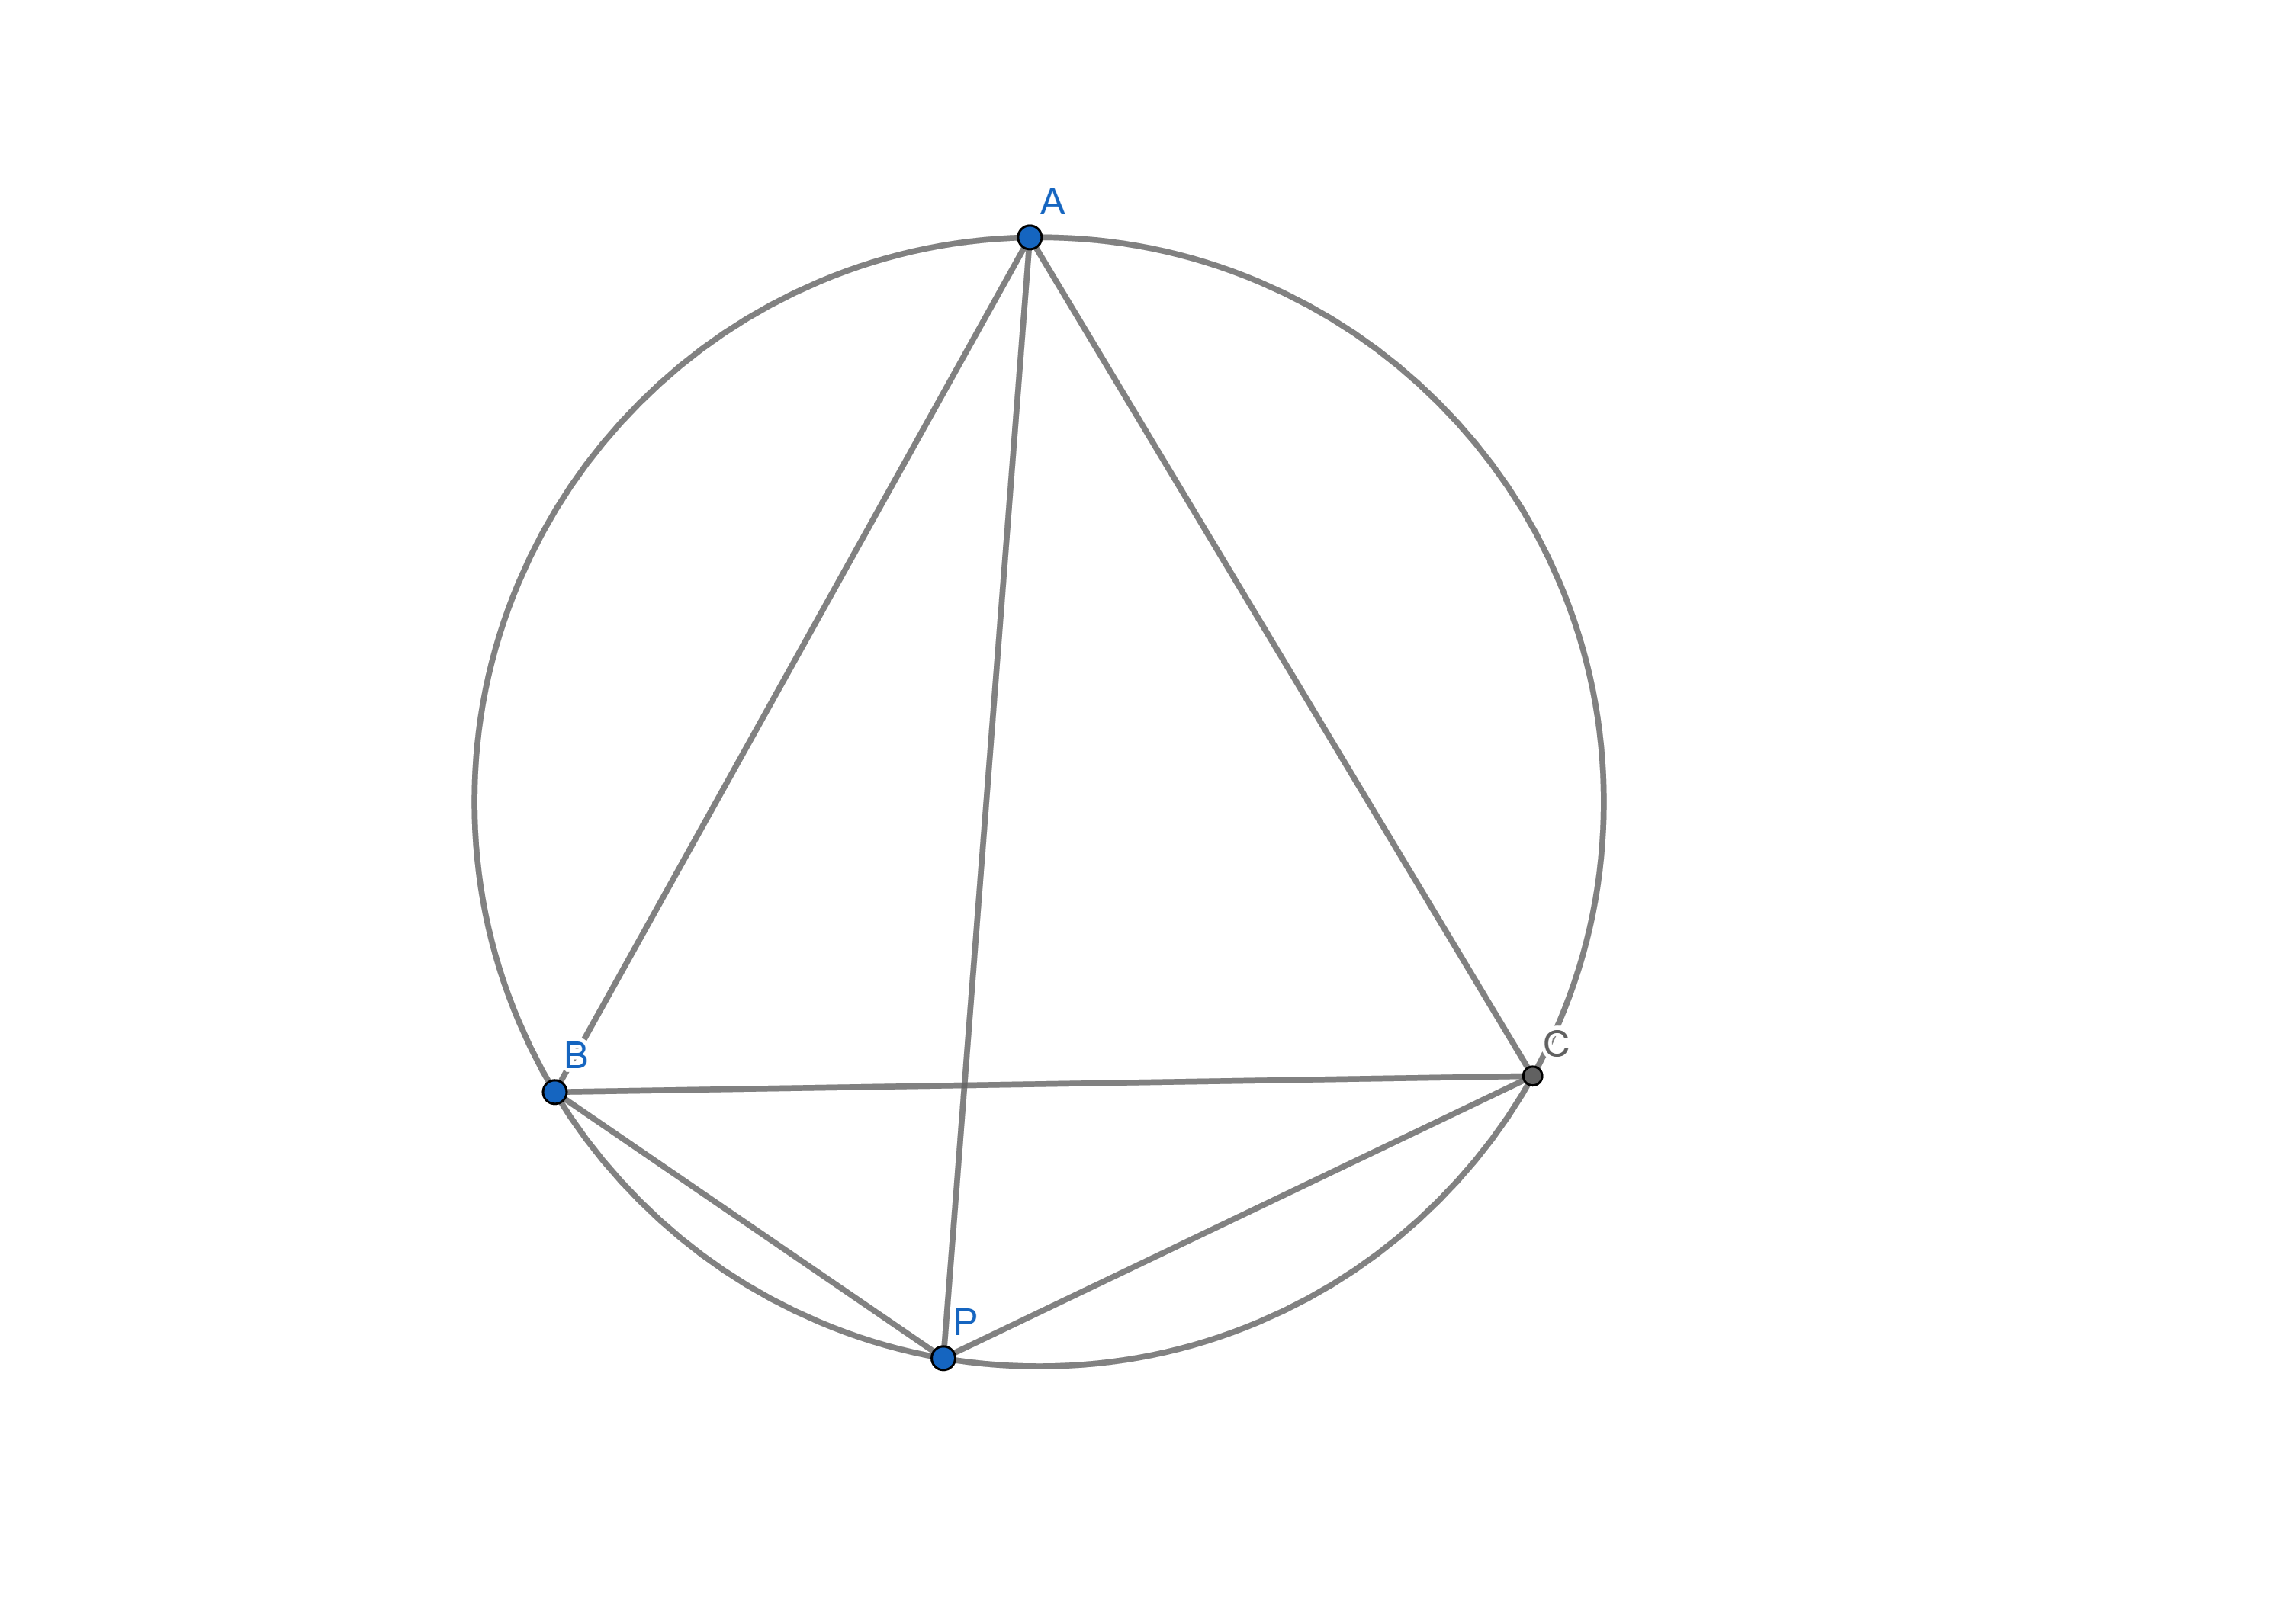
\includegraphics[scale=0.4]{q37-diagram}
\end{center}

\solution[37]{brainysmurfs}{281300961312374785}{
Suppose $\angle BAP = a$. Then $\angle CBP = 60 - a \implies \angle ACP = a \implies \angle BCP = 60 + a$. \\
By extended sine rule, 
\begin{equation}
$$\begin{align*}
PA &= 2R \sin \angle ABP\\
&= 2R \sin a\\
PB &= 2R \sin (60 + a) \\
&= 2R (\sin a \cos 60 + \cos a \sin 60)\\
&= 2R(\frac{1}{2}\sin a + \frac{\sqrt{3}}{2}\cos a)\\
PC &= 2R(\sin(60 - a))\\
&= 2R(\frac{\sqrt{3}}{2} \cos a - \frac{1}{2}\sin a)
\end{align*}$$\end{equation}
So, 
\begin{equation}
$$\begin{align*}
PA+PC &= 2R(\sin a - \frac{1}{2} \sin a + \frac{\sqrt{3}{2}} \cos a)\\
&= 2R(\frac{\sqrt{3}}{2} \cos a + \frac{1}{2} \sin a)\\
&= PB \\
\end{align*}$$
\end{equation}
as required. This finishes the proof. 
}

%May
\renewcommand{\themonth}{May}
\setcounter{datenumber}{1}

\anonsolution[37]{By applying Ptolemy's theorem on cyclic quadrilateral \(ABPC\), we find that \begin{align*} PA\cdot BC&= PB\cdot AC+PC\cdot AB \\ &= PB\cdot BC +PC\cdot BC \\ \iff PA&=PB+PC \end{align*} as desired, since \(AB=AC=BC\).}

\problem[38]{2007 Canadian MO (37th), Q2 of 5}{C4}{For two real numbers $a,b$ with $ab \neq 1$, define operation $\star$ by $a \star b = \frac{a + b - 2ab}{1 - ab}$. Start with a list of $n \geq 2$ real numbers that all satisfy $0 < x < 1$. Select any two numbers $a$ and $b$ in the list; remove them and put the number $a \star b$ at the end of the list, therefore reducing its length by 1. Repeat this procedure until a single number remains.\\
	(a) Prove that this single number is the same regardless of the choice of pair at each stage.\\
	(b) Suppose the condition on the numbers in the list is weakened to $0 < x \leq 1$. What happens if the list contains exactly one 1?}

\anonsolution[38]{We first show that for any \(0<x,y<1\), \(0<x\star y<1\). To prove \(0<x\star y\), note  

\begin{align*} 0&<\frac{x+y-2xy}{1-xy} \\ \iff x+y-2xy&>0 \\ \iff x+y&>2xy\end{align*} but since \(x,y\) are positive reals, \(x+y\geq 2\sqrt{xy}\). However, notice that for \(0<x,y<1\), \(\sqrt{xy}>xy\) because, in general for some positive constant \(c<1\), \(c>c^2\). Here, equality cannot hold because \(\sqrt{xy}=xy \implies xy=1\) which is not possible. Hence \(x+y\geq 2\sqrt{xy} > 2xy\), proving one direction. \\

Now to prove \(x\star y<1\), note that \begin{align*} \frac{x+y-2xy}{1-xy}&<1 \\ \iff x+y-2xy&<1-xy \\ \iff x+y-xy-1&<0 \\ \iff (x-1)(1-y)&< 0\end{align*} but this last inequality is obviously true, since \(x-1\) is always negative and \(1-y\) is always positive. So the set of reals between \(0\) and \(1\) is closed over \(\star\).  \\

Clearly, \(\star\) is commutative due to symmetry; we now prove that it is assosciative. For general \(0<x,y,z<1\) it is, while tedious, quite easy to compute that \[x \star (y\star z)=\frac{x+y+z-2xy-2xz-2yz+3xyz}{1-xy-xz-yz+2xyz} = (x\star y)\star z \] (the reader is invited to verify this if desired). Then any chain of \(\star\) operations performed on a list of reals (between \(0\) and \(1\)) is equivalent to any other rearrangement of the same chain of operations, so that the final result will always be the same. If the list contains exactly one \(1\), note that \(x\star 1=1\) for any \(x\neq 1\) and so the procedure will always end with the single number \(1\). } 

\problem[39]{C3}{2014 BMO1, Q3 of 6}{A hotel has ten rooms along each side of a corridor. An olympiad team leader wishes to book seven rooms on the corridor so that no two reserved rooms on the same side of the corridor are adjacent. In how many ways can this be done?}

\problem[40]{N5}{2002 IMO (43rd), Q4}{The positive divisors of the integer $n > 1$ are  $d_1 < d_2 < \dots < d_k$, so that $d_1 = 1, d_k = n$. Let $d = d_1d_2 + d_2d3 + \dots + d{k-1}d_k$. Show that $d < n^2$ and find all $n$ for which $d$ divides $n^2$.}

\problem[41]{A2}{2006 Romanian MO, 9th Form, Q1 of 4}{Find the maximum value of $\left(x^3+1\right)\left(y^3+1\right)$, where $x$ and $y$ are real numbers such that $x + y = 1$.}

\problem[42]{N3}{2008 Spanish MO, Q4 of 6}{Let $p$ and $q$ be two different prime numbers. Prove that there are two positive integers, $a$ and $b$, such that the arithmetic mean of the divisors of $n = p^a q^b$ is an integer.}

\problem[43]{G2}{2019 NZ Squad Selection Test, Q1}{The rectangle $ABCD$ has longest side $AB$. The point $E$ lies on the line $AD$ such that $BE$ is perpendicular to $AC$, and the point $F$ lies on the segment $CD$ such that $AF = AB$.\\Prove that the lines $AF$ and $EF$ are perpendicular.}

\problem[44]{C3}{2006 Flanders MO, Q3 of 4}{A total of 60 elves and trolls are seated around a table. Trolls always lie, and elves always speak the truth, except when they make a little mistake. Everybody claims to sit between an elf and a troll, but exactly two elves made a mistake! How many trolls are there at the table?}

\problem[45]{N6}{2017 IMO Shortlist, N2}{Let $p \geq 2$ be a prime number. Eduardo and Fernando play the following game making moves alternately: in each move, the current player chooses an index $i$ in the set ${0,1,\dots,p-1}$ that was not chosen before by either of the two players and then chooses an element $a_i$ of the set ${0,1,2,3,4,5,6,7,8,9}$. Eduardo has the first move. The game ends after all the indices $i \in {0,1,\dots,p-1}$ have been chosen. Then the following number is computed: \begin{equation}M = a_0 + 10\cdot a1 + \dots + 10^{p-1} \cdot a{p-1} = \sum_{j=0}^{p-1} a_j \cdot 10^j.\end{equation} The goal of Eduardo is to make the number $M$ divisible by $p$, and the goal of Fernando is to prevent this. Prove that Eduardo has a winning strategy.}

\problem[46]{A4}{2006 Flanders MO, Q4 of 4}{Find all functions $f:\mathbb{R}\setminus{0,1}\to\mathbb{R}$ such that \begin{equation}f(x) + f(\frac{1}{1-x})  = 1 + \frac{1}{x(1-x)}\end{equation} for all real $x$.}

\problem[47]{G4}{2009 Croatian TST, Q3 of 4}{Let $ABC$ be a triangle such that $AB > AC$. Let $l$ be a tangent at $A$ to the circumcircle of $ABC$. A circle with centre $A$ and radius $AC$ intersects $AB$ at $D$ and the line $l$ at $E$ and $F$ (in such a way that $C$ and $E$ are on the same side of $AB$). Prove that the line $DE$ passes through the incentre of $ABC$.}

\begin{center}
	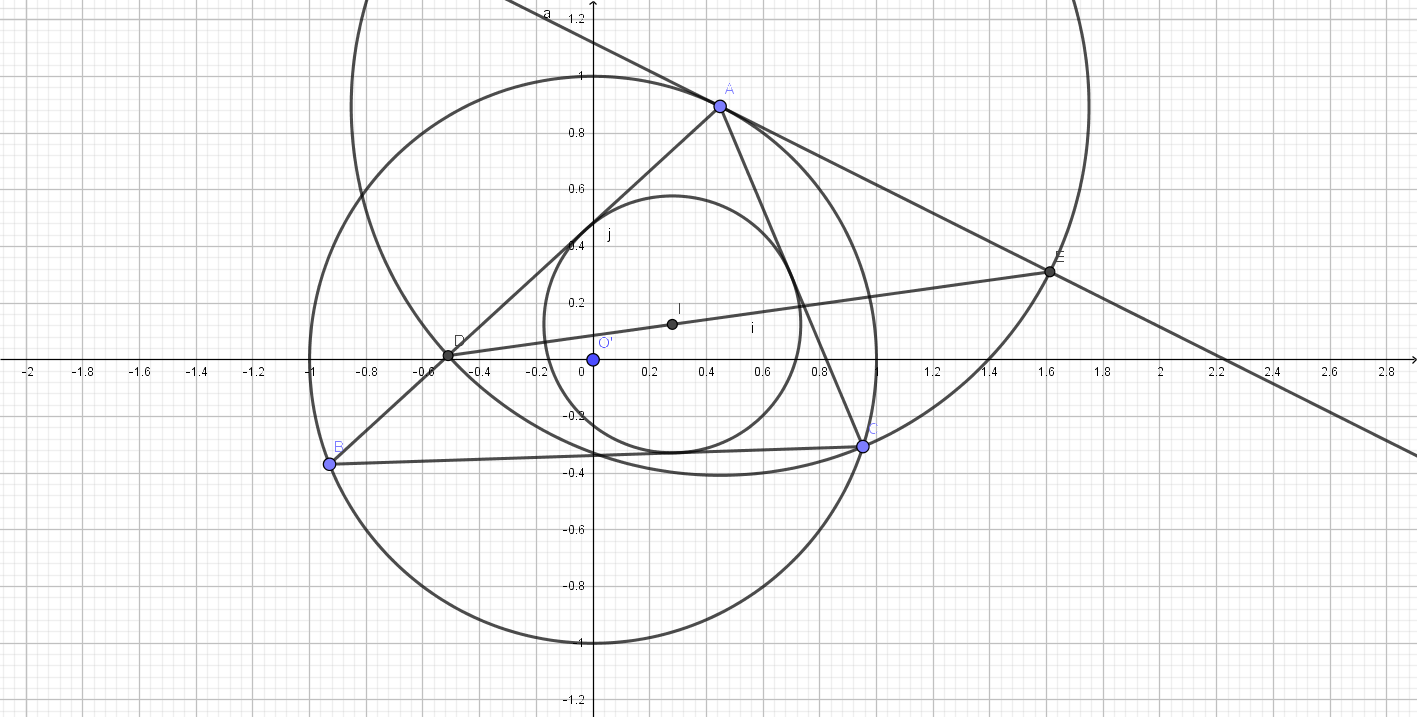
\includegraphics[scale=0.25]{q47-diagram}
\end{center}

\solution[47]{brainysmurfs}{281300961312374785}{Suppose $\angle BAC = 2a$, $\angle ABC = 2b$, $\angle ACB = 2c$. By Alternate Segment Theorem, $\angle EAC = 2b \implies \angle AEC = 90 - b$ by base angles in isosceles triangle. But it is well known that $\angle AIC = 90 + (\angle ABC)/2 = 90 + b$. So $AECI$ is cyclic. This means that $\angle IEC = \angle IAC = a$. By angles at center is twice angles on the circumference, we get that $\angle DEC = (\angle DAC)/2 = a$. Since $\angle IEC = \angle DEC$ we get that $DE$ passes through $I$.}

\problem[48]{CG3}{2009 Canada MO, Q5 of 5}{A set of points is marked on the plane, with the property that any three marked points can be covered with a disk of radius 1. Prove that the set of all marked points can be covered with a disk of radius 1.}

\problem[49]{C5}{2015 IMO Shortlist, C1}{In Lineland there are \(n \geq 1\) towns, arranged along a road running from left to right. Each town has a left bulldozer (put to the left of the town and facing left) and a right bulldozer (put to the right of the town and facing right). The sizes of the \(2n\) bulldozers are distinct. Every time when a right and a left bulldozer confront each other, the larger bulldozer pushes the smaller one off the road. On the other hand, the bulldozers are quite unprotected at their rears; so, if a bulldozer reaches the rear-end of another one, the first one pushes the second one off the road, regardless of their sizes.
	
	\quad Let \(A\) and \(B\) be two towns, with \(B\) being to the right of \(A\). We say that town \(A\) can sweep town \(B\) away if the right bulldozer of \(A\) can move over to \(B\) pushing off all bulldozers it meets. Similarly, \(B\) can sweep \(A\) away if the left bulldozer of \(B\) can move to \(A\) pushing off all bulldozers of all towns on its way.
	
	\quad Prove that there is exactly one town which cannot be swept away by any other one.}

\problem[50]{N3}{2014 BMO2, Q3 of 4}{Let $a_0 = 4$ and define a sequence of terms using the formula $an = a{n-1}^2 - a_{n-1}$ for each positive integer $n$.\
	a) Prove that there are infinitely many prime numbers which are factors of at least one term of the sequence.\
	b) Are there infinitely many prime numbers which are factors of no term in the sequence?}

\problem[51]{A3}{2008 Polish MO Round 1, Q9 of 12}{Determine the smallest real number $a$ having the following property: For any real numbers $x,y,z \geq a$ satisfying $x+y+z = 3$, it holds that $x^3 + y^3 + z^3 \geq 3$.}

\problem[52]{G3}{2000 Mexico MO, Q6 of 6}{Let $ABC$ be a triangle with $\angle B > 90^{\circ}$ such that there is a point $H$ on side $AC$ with $AH = BH$ and $BH$ perpendicular to $BC$. Let $D$ and $E$ be the midpoints of $AB$ and $BC$ respectively. A line through $H$ parallel to $AB$ cuts $DE$ at $F$. Prove that $\angle BCF = \angle ACD$.}

\problem[53]{C4}{2019 NZ Squad Selection Test, Q7 of 9}{A set $S$ of positive integers is \textit{self-indulgent} if $\gcd (a, b) = \vert a - b \vert$ for any two distinct $a, b \in S$. \begin{itemize} \item[(a)] Prove that any self-indulgent set is finite. \item[(b)] Prove that for any positive integer n, there exists a self-indulgent set with at least n elements. \end{itemize}}

\anonsolution[53]{
\begin{itemize}
	\item[(a)] Let $a_1$ be the smallest element of the set. Let $a_n$ be the largest element of the set. Since $a_n - a_0 = gcd(a_0, a_n) \leq a_0$ we have that $a_n \leq 2a_0$. So each self-indulgent set is bounded above by twice its smallest element, so is necessarily finite. 
	\item[(b)] Note that the following sets are self-indulgent for the various values of $n$:
		\begin{itemize}
			\item[n=1:] {1}
			\item[n=2:] {5,10}
			\item[n=3:] {6,8,9}
			\item[n=4:] {8,9,10,12}
		\end{itemize}
	We prove this result for all $n \geq 4$ by induction on $n$. \\
	\paragraph{Base case ($n=4$)} is taken care of earlier. \\
	\paragraph{Inductive step:}
	Let $\{a_1, a_2, a_3, \dots , a_n\}$ be a self-indulgent set with $n$ elements. We claim that the set $\{b_0, b_1, b_2, \dots , b_n\}$ is also self-indulgent with $n+1$ elements, where $b_0 = \lcm(a_1, a_2, \dots a_n)$ and $b_i=a_i+b_0$ $\forall$ $0 < i \leq n$. Then it is trivial to note this new set is also self-indulgent. 
\end{itemize}}

\problem[54]{A2}{2018 Putnam, Q1 of 12}{Find all ordered pairs of integers $(a,b)$ for which $$\frac{1}{a}+\frac{1}{b}= \frac{3}{2018}$$}

\problem[55]{G4}{2016 APMO, Q1 of 5}{We say that a triangle $ABC$ is great if the following holds: for any point $D$ on the side $BC$, if $P$ and $Q$ are the feet of the perpendiculars from $D$ to the lines $AB$ and $AC$, respectively, then the reflection of $D$ in the line $PQ$ lies on the circumcircle of the triangle $ABC$. Prove that triangle $ABC$ is great if and only if $\angle A = 90^{\circ}$ and $AB = AC$.}

\problem[56]{G4}{2013 APMO, Q3 of 5}{Let $ABCD$ be a quadrilateral inscribed in a circle $\omega$, and let $P$ be a point on the extension of $AC$ such that $PB$ and $PD$ are tangent to $\omega$. The tangent at $C$ intersects $PD$ at $Q$ and the line $AD$ at $R$. Let $E$ be the second point of intersection between $AQ$ and $\omega$. Prove that $B$, $E$, $R$ are collinear.}

\problem[57]{A2}{2011 BMO1, Q1 of 6}{Find all \emph{positive or negative} integers for which $n^2+20n+11$ is a perfect square. \textit{Remember that you must justify that you have found them all.}}

\problem[58]{G4}{2016 BMO2, Q3 of 4}{Consider the cyclic quadrilateral \(ABCD\). The diagonals \(AC\) and \(BD\) meet at \(P\), and the rays \(AD\) and \(BC\) intersect at \(Q\). The internal angle bisector of \(\angle BQA\) meets \(AC\) at \(R\) and the internal angle bisector of \(\angle APD\) meets \(AD\) at \(S\). Prove that \(RS\) is parallel to \(CD\).}

\problem[59]{C2}{2019 New Zealand Squad Selection Test, Q2 of 8}{Andrew chooses a set $A$ of 100 different points in the plane, no three of them collinear. Show that amongst the triangles with all their vertices in $A$, there are at least 100 that are not equilateral.}

\problem[60]{A3}{2017 Australian MO, Q5 of 8}{Determine the number of positive integers (n) less than 1000000 for which the sum \[\frac{1}{2 \times \lfloor \sqrt{1} \rfloor + 1} + \frac{1}{2 \times \lfloor \sqrt{2} \rfloor + 1} + \cdots +\frac{1}{2 \times \lfloor \sqrt{n} \rfloor + 1}\] is an integer.}

\problem[61]{N3}{Monday Maths Workshop Feb 2019, Q6 of 8}{Show that there are infinitely many integer solutions $(x, y)$ to the equation \[x^2-3y^2=1.\]}

\problem[62]{G8}{2018 Sharygin Q15}{The altitudes $AH_1,BH_2,CH_3$ of an acute-angled triangle $ABC$ meet at point $H$. Points $P$ and $Q$ are the reflections of $H_2$ and $H_3$ with respect to $H$. The circumcircle of triangle $PH_1Q$ meets for the second time $BH_2$ and $CH_3$ at points $R$ and $S$. Prove that $RS$ is a medial line of triangle $ABC$.}

\problem[63]{C4}{Some Australian TST}{Players Dan and Daniel take turns in putting the numbers $1$ to $64$ (not necessarily in that order) into the squares of an $8 \times 8$ chess board, with Dan going first. At the end the smallest number in each column is circled. Then the sum $S$ of the circled numbers is calculated.
	
	\begin{enumerate}
		\item[(a)] Can Daniel always play in such a way that $S$ is even?
		
		\item[(b)] Can Daniel always play in such a way that $S$ is odd?
	\end{enumerate}}

\problem[64]{C3}{2017 Russian MO National Finals, Day 1}{In a country, some cities are connected by one-way flights. (There is no more than one flight between two cities.) City \(A\) is said to be ``available'' for city \(B\) if there are flights (not necessarily directly) from \(B\) to \(A\). It is known that for any 2 cities \(P\) and \(Q\), there is a city \(R\) such that both \(P\) and \(Q\) are available from \(R\). Prove there is a city \(A\) such that every city is available for \(A\).}

\problem[65]{A5}{1995 IMO Q2 of 6}{Let $a$, $b$, $c$ be positive real numbers such that $abc=1$. Prove that \[\frac{1}{a^3(b+c)} + \frac{1}{b^3(c+a)} + \frac{1}{c^3(a+b)} \geq \frac{3}{2}.\]}

\problem[66]{Cg8}{2017 USAMO P5 of 6}{Let \(\mathbb{Z}\) denote the set of all integers. Find all real numbers \(c > 0\) such that there exists a labeling of the lattice points \(( x, y ) \in \mathbb{Z}^2\) with positive integers for which: only finitely many distinct labels occur, and for each label \(i\), the distance between any two points labeled \(i\) is at least \(c^i\).}

\problem[67]{N2}{Tournament of Towns Spring 2004 Junior O-level Q4}{A positive integer $a > 1$ is given (in decimal notation). We copy it twice and obtain a number $b = \overline{aa}$ which happens to be a multiple of $a^2$. Find all possible values of $\frac{b}{a^2}$.}

%June
\renewcommand{\themonth}{June}
\setcounter{datenumber}{1}

\problem[68]{G3}{2018 BMO2, Q1 of 4}{Consider triangle \(ABC\). The midpoint of \(AC\) is \(M\). The circle tangent to \(BC\) and \(B\) and passing through \(M\) meets the line \(AB\) again at \(P\). Prove that \(AB\times BP=2BM^2\).}

\problem[69][G3]{2019 EGMO, Q4 of 6}{Let \(ABC\) be a triangle with incenter \(I\). The circle through \(B\) tangent to \(AI\) at \(I\) meets side \(AB\) again at \(P\). The circle through \(C\) tangent to \(AI\) at \(I\) meets side \(AC\) again at \(Q\). Prove that \(PQ\) is tangent to the incircle of \(ABC\). }

\problem[70]{C2}{One of those ``99\% cannot solve'' quizzes}{Brainy is trying to create a jewelled string by following some rules. He begins with a ruby on a the string. With his string, he has 4 possible operations he could do:
	\begin{enumerate}
		\item He could add a sapphire gem to the end of the string.
		\item He could make a copy of the string he has and add it on to the end of his initial string.
		\item He could replace any three contiguous ruby gems with a sapphire.
		\item He can remove any two consecutive sapphire.
	\end{enumerate}
	Is it possible to make the string have only a sapphire on it?}

\problem[71]{N3}{1989 APMO, Q2 of 5}{Prove that the equation \[6(6a^2+3b^2+c^2)=5n^2\] has no solutions in integers except $a=b=c=n=0$.}

\problem[72]{A8}{2018 NZ Camp Selection Problems, Q10 of 10}{Find all functions $f : \mathbb{R} \to \mathbb{R}$ such that \[f(x)f(y) = f(xy+1)+f(x-y)-2\] for all $x, y \in \mathbb{R}.$}

\problem[73]{N3}{2011 BMO2, Q2 of 4}{Find all positive integers $x$ and $y$ such that $x+y+1$ divides $2xy$ and $x+y-1$ divides $x^2+y^2-1$. }

\problem[74]{C3}{1971 Putnam, A1}{Let there be given nine lattice points in 3-dimensional space. Show that there is a lattice point on the interior of one of the line segments joining two of these points.}

\problem[75]{G4}{2018 APMO, Q1 of 5}{Let $H$ be the orthocenter of the triangle $ABC$. Let $M$ and $N$ be the midpoints of the sides $AB$ and $AC$, respectively. Assume that $H$ lies inside the quadrilateral $BMNC$ and that the circumcircles of triangles $BMH$ and $CNH$ are tangent to each other. The line through $H$ parallel to $BC$ intersects the circumcircles of the triangles $BMH$ and $CNH$ in the points $K$ and $L$, respectively. Let $F$ be the intersection point of $MK$ and $NL$ and let $J$ be the incenter of triangle $MHN$. Prove that $FJ = FA$.}

\problem[76]{Cg2}{2006 Irish MO (19th), Part I, Q3 of 5}{Prove that a square of side 2.1 units can be completely covered by seven squares of side 1 unit.}

\problem[77]{G2}{2014 New Zealand Camp Selection Problems, Q2}{Let $ABC$ be a triangle in which the length of side $AB$ is $4$ units, and that of $BC$ is $2$ units. Let $D$ be the point on $AB$ at distance $3$ units from $A$. Prove that the line perpendicular to $AB$ through $D$, the angle bisector of $\triangle ABC$, and the perpendicular bisector of $BC$ all meet at a single point.}

\problem[78]{A2}{1983 Yugoslav Federal MC (24th), Grade 3/4, Q2 of 4}{A function \(f\) is defined on the integers and satisfies \[ f(x) = \begin{cases} x-10, & \text{if } x > 100,\\ f(f(x+11)), & \text{if } x \leq 100. \end{cases}\]
	Prove that \(f(x) = 91\) for all \(x \leq 100\).}

\problem[79]{C2}{2017 Kosovo National Olympiad, Grade 11, Q3 of 4}{\(n\) teams participated in a basketball tournament, where each team played with each other team exactly one game. There was no tie. If in the end of the tournament the \(i\)-th team has \(W_i\) wins and \(L_i\) losses for \(1 \leq i \leq n\) prove that
	\[\displaystyle \sum_{i=1}^n W_i^2 = \displaystyle \sum_{i=1}^n L_i^2.\]}

\problem[80]{A2}{2015 Australian Intermediate Math Olympiad, Q8}{Determine the number of non-negative integers \(x\) that satisfy the equation \[\left \lfloor \frac{x}{44}  \right\rfloor  = \left \lfloor \frac{x}{45} \right \rfloor .\]
	(\textit{Note: if \(r\) is any real number, then \(\lfloor r \rfloor\) denotes the largest integer less than or equal to \(r\)}.)}

\problem[81]{N3}{2015 Singapore Maths Olympiad Junior R2, Q5}{Find all positive integers \(k\) such that \(k^k+1\) is divisible by \(30\). Justify your answer. }

\problem[82]{N4}{2016 NZ Camp Selection Problems, Q7}{Find all positive integers \(n\) for which the equation \[(x^2+y^2)^n = (xy)^{2016}\] has positive integer solutions. }

\problem[83]{C7-8}{2011 USAMO, Q6}{Let $\mathcal{A}$ be a set with $225$ elements. Suppose further that there are eleven subsets of $\mathcal{A}$ such that each $\mathcal{A}_i$ has $45$ elements, and $\vert \mathcal{A}_j \cap \mathcal{A}_j \vert = 9 $ $\forall$ $ 1 \leq i < j \leq 11$. Prove that $\vert \mathcal{A}_1 \cup \mathcal{A}_2 \cup\cdots \cup \mathcal{A}_{11} \vert \geq 165$, and give an example for which equality holds. }

\problem[84]{C4}{1991 Asian Pacific Mathematical Olympiad, Q2}{Suppose there are $997$ points given in a plane. If every two points are joined by a line segment with its midpoint coloured in red, show that there are at least $1991$ red points in the plane. Can you find a special case with exactly $1991$ red points?}

\problem[85]{G3}{2002 Japanese MO, Q1}{Distinct points $A$, $M$, $B$ with $AM=MB$ are given on a circle $C_0$. Let $P$ be a point on the arc $AB$ not containing $M$. Circle $C_1$ is internally tangent to $C_0$ at $P$ and tangent to $AB$ at $Q$. Prove that the product $MP \times MQ$ is independent of the position of $P$. }

\problem[86]{C3}{2014 British Mathematical Olympiad R2, Q1}{Every diagonal of a regular polygon with $2014$ sides is coloured in one of $n$ colours. Whenever two diagonals cross in the interior, they are of different colours. \\
	What is the minimum value of $n$ for which this is possible?}

\problem[87]{N2}{1998 Asian Pacific Mathematical Olympiad, Q2}{Show that for any two positive integers \(a\) and \(b\), \((36a+b)(a+36b)\) cannot be a power of 2. }

\problem[88]{A4}{2017 Singapore MO Senior Division R2, Q4}{Find all functions $f : \mathbb{Z}^{+} \to \mathbb{Z}^{+}$ such that $f(k+1) > f(f(k))$ for all $k \geq 1$, where $\mathbb{Z}^{+}$ is the set of positive integers. }

\problem[89]{Cg4}{2018 NZ Camp Selection Problems, Q6}{The intersection of a cube and a plane is a pentagon. Prove that the length of at least one side of the pentagon differs from 1 metre by at least 20 centimetres. }

\problem[90]{N3}{2017 Singapore MO Open Round 2, Q3}{Find the smallest integer $n$ so that $\sqrt{\frac{1^2+2^2+3^2+ \cdots + n^2}{n}}$ is an integer. (and $n > 1$)}

\problem[91]{G4}{2000 Belarus Team Selection Test 8, Q1}{The diagonals of a convex quadrilateral \(ABCD\) with \(AB = AC = BD\) intersect at \(P\), and \(O\) and \(I\) are the circumcentre and incentre of triangle \(ABP\), respectively. Prove that if \(O \neq I\) then \(OI\) and \(CD\) are perpendicular.}

\problem[92]{A3}{2009 Moldova TST2, Q2}{Determine all functions \(f\) from the non-negative reals to the non-negative reals such that
	\[f\left(x+y-z\right) + f\left(2\sqrt{xz}\right) + f\left(2\sqrt{yz}\right) = f\left(x+y+z\right)\]
	for all real \(x,y,z \geq 0\) such that \(x + y \geq z\).}

\problem[93]{N2}{2010 Spanish MO Day 1, Q1}{A \textit{pucelana} sequence is an increasing sequence of 16 consecutive odd numbers whose sum is a perfect cube. How many pucelana sequences are there with 3-digit numbers only?}

\problem[94]{Cg3}{2007 Mongolian MO Secondary, Q2}{Given 101 segments on a line, prove that there either exists a point contained in at least 11 of the segments, or at least 11 segments that are pairwise disjoint.}

\problem{A2}{2019 NZ Senior Math Comp Prelim Round, Q10}{Solve the following equation, giving exact solutions. 
	\[\sqrt[3]{5-x} + \sqrt[3]{5+x}=\sqrt[3]{25}.\]}

\problem{C6}{2004 Niels Henrik Abel Contest (Norway), P4}{Among the \(n\) inhabitants of an island, where \(n\) is even, every two are either friends or enemies. One day, the chief of the island orders that each inhabitant (including himself) makes and wears a necklace consisting of marbles, in such a way that two necklaces have a marble of the same type if and only if their owners are friends.
	\begin{enumerate}
		\item[(a)] Show that the chief’s order can be achieved by using \(n^2/4\) different types of marbles.
		\item[(b)] Prove that this is not necessarily true with less than \(n^2/4\) types of marbles.
	\end{enumerate}}

\problem{G3}{2001 Croatian TST, Q2}{
Circles \(k_1\) and \(k_2\) intersect at \(P\) and \(Q\), and \(A\) and \(B\) are the tangency points of their common tangent that is closer to \(P\) (where \(A\) is on \(k_1\) and \(B\) is on \(k_2\)). The tangent to \(k_1\) at \(P\) intersects \(k_2\) again at \(C\). The lines \(AP\) and \(BC\) meet at \(R\). Show that the lines \(BP\) and \(BC\) are tangent to the circumcircle of triangle \(PQR\).}

%July
\renewcommand{\themonth}{July}
\setcounter{datenumber}{1}

\problem[98]{A3}{2009 Hungary-Israel Binational, Q2}{Denote the three real roots of the cubic \(x^3 - 3x - 1 = 0\) by \(x_1, x_2,\) and \(x_3,\) with \(x_1 < x_2 < x_3\). Prove that \(x_3^2 - x_2^2 = x_3 - x_1.\)}

\problem[99]{N3}{2001 Polish MO, Round 1, Q5}{Prove that for all integers \(n \geq 2\) and all prime numbers \(p\), the number \(n^{p^p} + p^p\) is composite.}

\problem[100]{N6}{2016 IMO, Problem 4}{A set of positive integers is called \textit{fragrant} if it contains at least two elements and each of its elements has a prime factor in common with at least one of the other elements. Let \(P(n) = n^2 + n + 1.\) What is the least possible value of the positive integer \(b\) such that there exists a non-negative integer \(a\) for which the set
	\[\{P\left(a+1\right), P\left(a+2\right), \dots, P\left(a+b\right)\}\]
	is fragrant?}

\problem[101]{G7}{Asian Pacific MO, Q3}{Let \(ABC\) be a scalene triangle with circumcircle $\Gamma{}$. Let \(M\) be the midpoint of \(BC\). A variable point \(P\) is selected in the line segment \(AM\). The circumcircles of triangles $BPM$ and $CPM$ intersect$ \Gamma{}$ again at points $D$ and $E$, respectively. The lines $DP$ and $EP$ intersect (at second time) the circumcircles to triangles $CPM$ and $BPM$ at $X$ and $Y$, respectively. Prove that as $P$ varies, the circumcircle of $\triangle AXY$ passes through a fixed point $T$ distinct from $A$. }

\problem[102]{Cg6}{2013 IMO Shortlist, C2}{In the plane, 2013 red points and 2014 blue points are marked so that no three of the marked points are collinear. One needs to draw \(k\) lines not passing through the marked points and dividing the plane into several regions. The goal is to do it in such a way that no region contains points of both colors.\\
	Find the minimal value of \(k\) such that the goal is attainable for every possible configuration of 4027 points.}

\problem[103]{Cg3}{2019 Australian MO, Q4}{Let \(Q\) be a point inside the convex polygon \(P_1 P_2 \dots P_{1000}\). For each \(i=1, 2, \dots, 1000\), extend the line \(P_i Q\) until it meets the polygon again at a point \(X_i\). Suppose that one of the points \(X_1, X_2, \dots, X_{1000}\) is a vertex of the polygon.\\
\makebox[16pt]{}Prove that there is at least one side of the polygon that does not contain any of the points \(X_1, X_2, \dots, X_{1000}\).}

\problem[104]{N4}{2018 Tournament of Towns, Senior Q3}{Prove that\\
	\begin{enumerate}
		\item any integer of the form \(3k-2\), where \(k\) is an integer, can be represented as the sum of a perfect square and two perfect cubes of some integers.
		\item any integer can be represented as the sum of a perfect square and three perfect cubes of some integer.
	\end{enumerate}}

\problem[105]{A5}{2006 Indian MO, Q5}{Let \(ABC\) be a triangle with sides \(a, b, c\), circumradius \(R\), and inradius \(r\). Prove that
	\[\frac{R}{2r} \geq \left ( \frac{64a^2b^2c^2}{(4a^2-(b-c)^2)(4b^2-(c-a)^2)(4c^2-(a-b)^2)} \right )^2.\]}

\problem[106]{G4}{2008 Japan MO, Q3}{Suppose there exists an acute-angled triangle \(ABC\) with circumcentre \(O\). A circle passing through \(A\) and \(O\) intersects lines \(AB\) and \(AC\) at \(P\) and \(Q\) respectively, distinct from \(A\). Suppose \(PQ\) and \(BC\) are equal in length. Find the possible angles \(\leq 90^{\circ}\) created between \(PQ\) and \(BC\).}

\problem[107]{A3}{2004 British MO Round 2, Q3}{\begin{itemize}
		\item[(a)] Given real numbers $a$, $b$ and $c$ with $a+b+c=0$, prove that $a^3+b^3+c^3>0$ iff $a^5+b^5+c^5>0$. 
		\item[(b)] Given real numbers $a$, $b$, $c$ and $d$ with $a+b+c+d=0$, prove that $a^3+b^3+c^3+d^3>0$ iff $a^5+b^5+c^5+d^5>0$.
	\end{itemize}}

\problem[108]{G5}{2018 USA TSTST, Q5}{Let \(ABC\) be an acute triangle with circumcircle \(\omega\), and let \(H\) be the foot of the altitude from \(A\) to \(\overline{BC}\). Let \(P\) and \(Q\) be the points on \(\omega\) with \(PA = PH\) and \(QA = QH\). The tangent to \(\omega\) at \(P\) intersects lines \(AC\) and \(AB\) at \(E_1\) and \(F_1\) respectively; the tangent to \(\omega\) at \(Q\) intersects lines \(AC\) and \(AB\) at \(E_2\) and \(F_2\) respectively. Show that the circumcircles of \(\triangle AE_1F_1\) and \(\triangle AE_2F_2\) are congruent, and the line through their centres is parallel to the tangent to \(\omega\) at \(A\).}

\problem[109]{C3}{2017 BMO1 Q5}{If we take a \(2 \times 100\) (or \(100 \times 2\)) grid of unit squares, and remove alternate squares from a long side, the remaining 150 squares form a \textit{100-comb}. Henry takes a \(200 \times 200\) grid of unit squares, and chooses \(k\) of these squares so that James is unable to choose 150 uncoloured squares which form a 100-comb. What is the smallest possible value of \(k\)?}

\problem[110]{A5}{2018 Mathematical Ashes, P2}{Let \(\mathbb{N}_0\) denote the set of non-negative integers. Find all functions \(f:\mathbb{N}_0\to\mathbb{N}_0\) such that
	\[f^{f(m)}(n) = n + 2f(m)\]
	for all \(m,n \in \mathbb{N}_0\) with \(m \leq n\).}

\problem[111]{G3}{2000 Swiss TST, P1}{A convex quadrilateral \(ABCD\) is inscribed in a circle. Show that the line connecting the midpoints of the arcs \(AB\) and \(CD\) and the line collecting the midpoints of the arcs \(BC\) and \(DA\) are perpendicular.}

\problem[112]{Cg4}{2018 Canadian MO, P1}{Consider an arrangement of tokens in the plane, not necessarily at distinct points. We are allowed to apply a sequence of moves of the following kind: Select a pair of tokens at points A and B and move both of them to the midpoint of A and B.\\
	We say that an arrangement of \(n\) tokens is \textit{collapsible} if it is possible to end up with all \(n\) tokens at the same point after a finite number of moves. Prove that every arrangement of \(n\) tokens is collapsible if and only if \(n\) is a power of 2.}

\end{document}
